\documentclass[10pt,twoside]{fernandes_supp} 
%Default opts:9pt,twocolumn,twoside
\graphicspath{{images_supp/}}

\newcommand{\KB}[1]{\noindent\color{blue}$\Longrightarrow$ #1\normalcolor}
\newcommand{\mf}[1]{\colorbox{blue!10}{\color{color3}#1}}

\title{Supplemental Information:\\ Harnessing  Design Principles from Glass Sponges for Structurally Robust Lattice Structures}

\author[1]{Matheus C. Fernandes}
\author[2]{James C. Weaver}
\author[1,3,*]{Katia Bertoldi}

\affil[1]{John A. Paulson School of Engineering and Applied Sciences -- Harvard University, Cambridge, MA 02138}
\affil[2]{Wyss Institute -- Harvard University, Cambridge, MA 02138}
\affil[3]{Kavli Institute -- Harvard University, Cambridge, MA 02138}
\affil[*]{Corresponding author: \href{mailto:bertoldi@seas.harvard.edu}{bertoldi@seas.harvard.edu}}

\begin{document}
\maketitle
% \doublespace
% \linenumbers
\section{Structure of the Hexactinellid sponge \textit{Euplectella aspergillum}}\label{sec:params}
The periodic structures investigated in this study are inspired by the skeleton of the Hexactinellid sponge \textit{Euplectella aspergillum (sp.)}, commonly known as the "Venus' flower basket". In this section we provide a detailed description of the sponge geometry and measured dimensions.

\Cref{Sponge} shows a photograph of the entire skeleton of the \textit{Euplectella sp.}, and its intricate, cylindrical cage-like structure (20 to 25cm long, 2 to 4 cm in diameter) \citep{aizenberg2005}. The surface of the cylinder consists of a regular square lattice composed of a series of cemented vertical and horizontal struts with circular cross-section. The cell spacing between horizontal and vertical struts was reported  to be $L\approx 2.5$mm \citep{weaver2007}, while their diameter was measured to be $D_{nd}\approx 0.25$mm \citep{weaver2007}. Besides the horizontal and vertical struts, there is an additional set of diagonal elements, intersecting in a manner that creates a series of alternating open and closed cells, reminiscent of a checkerboard pattern \citep{weaver2007}. Although these diagonal elements are not as ordered as the horizontal and vertical ones, it has been shown that they can be approximated with two diagonal struts that are offset from the nodes  (vertex joints between non-diagonal elements) and form octagonal openings (\cref{Sponge}(d)). To estimate the volume ratio between diagonal and non-diagonal elements, we took high resolution photographs of the sponge and performed image segmentation to segregate the projected area of the vertical/horizontal and diagonal spicules. Using this approach, the projected area ratio of non-diagonal to diagonal elements was found to be $A_{nd}/A_{d}\approx1.4$. Note that here, and in the following, the subscripts $d$ and $nd$ are used to indicate diagonal and non-diagonal (i.e. horizontal and vertical) elements, respectively. 

Finally, it should also be noted that the sponge is reinforced by external ridges that extend perpendicular to the surface of the cylinder and spiral the cage at an angle of $45^\text{o}$. However, in this paper we do not report the effects of these ridges on it's structural performance.

\begin{figure}[H]
    \centering
    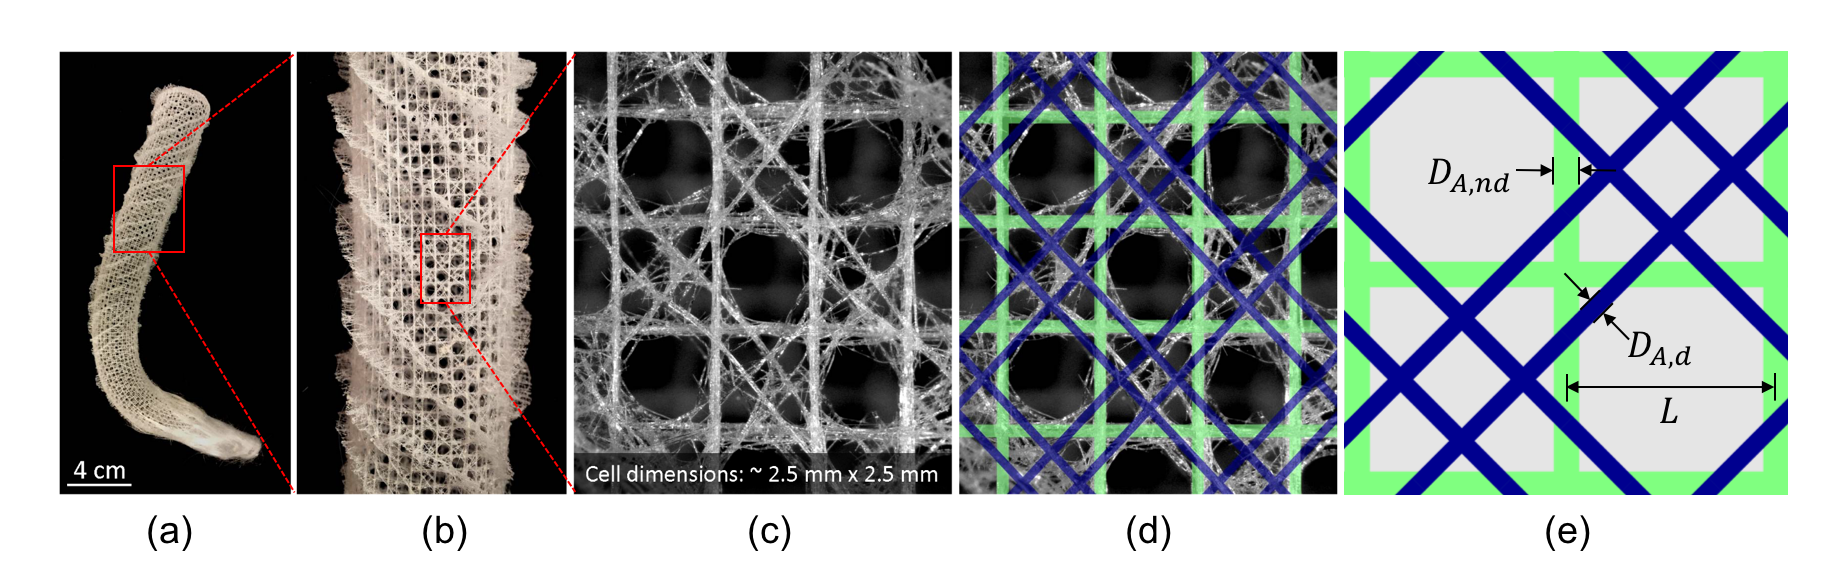
\includegraphics[width=0.9\linewidth]{SFig1.png}
    \caption{\textbf{Hexactinellid sponge \textit{Euplectella aspergillum.}} (a)-(b) Full-frame photo of sponge.  (c)  Close up microscope image of the sponge. (d) Comparison between the idealized model (green and blue lines) and the sponge structure. (e) Unit cell of the idealized model.}
    \label{Sponge}
\end{figure}

\section{Designs Considered}\label{sec:designs}
In this study, we focus on four different lattice configurations constrained to deform in an in-plane setting only. In an effort to conduct a fair performance comparison between the different designs, the total volume of material is conserved. Moreover,  we consider a fixed volume ratio between non-diagonal and diagonal elements (chosen to match the sponge geometry) as well as two different shapes for the cross section of all lattice members: circular and rectangular.  For the circular cross-section case  we stay consistent with the geometry found within the biological species. However, since slender members with such cross-section easily buckle out-of-plane when subject to compression loading we mitigate the issue by pursuing a plane-strain representative structure. To do so, we introduce the rectangular cross-section, where it's depth to slenderness ratio is sufficiently large to avoid out-of-plane deformation. 

In the subsequent sections, we describe in detail the unit cells for four different designs (Designs A-D), and provide the derivations for each geometry cross-section values. 

\subsection{Design A}
Design A is inspired by the sponge structure and consists of a square grid  reinforced by a double diagonal system (see \cref{DesignA}). 
\subsubsection{Circular cross section} 
If we assume that the horizontal and vertical struts have length $L$ and circular cross section  with diameters $D_{A,nd}$, their volume and projected-area in the unit cell are given by 
\begin{equation}\label{V1}
V_{A,nd}=8 L \left(\pi\frac{D^2_{A,nd}}{4}\right)=2 L \pi D^2_{A,nd}
\end{equation}
and
\begin{equation}\label{A1}
A_{A,nd}=8 L D_{A,nd},
\end{equation}
respectively. Note that in this study we use 
\begin{equation}
\frac{D_{A,nd}}{L}=0.1,
\end{equation}
since this is the aspect ratio measured for the sponges (see \cref{sec:params}).

Moreover, as for the case of the sponge, the diagonal elements are assumed to form an octagonal opening on every other cell. As such, the diagonals intersect the horizontal and vertical struts at a distance $\Delta L=L/(\sqrt{2}+2)$ from the nodes and their  volume and projected area in the unit cell are
\begin{equation}\label{V2}
V_{A,d}=8 \sqrt{2} L\left(\pi\frac{D^2_{A,d}}{4}\right)=2\sqrt{2}L \pi D^2_{A,d},
\end{equation}
and
\begin{equation}\label{A2}
A_{A,d}=8\sqrt{2} L D_{A,d},
\end{equation}
respectively. Since the projected area ratio of the non-diagonal to diagonal elements in the sponge has been measured to be 
\begin{equation}
\frac{A_{A,nd}}{A_{A,d}}=1.4,
\end{equation}
by substituting \cref{A1} and \cref{A2} into the equation above we find that for Design A
\begin{equation} \label{DA}
D_{A,nd}=1.4\sqrt{2}D_{A,d}\approx 2 D_{A,d}.
\end{equation}
Substitution of \cref{DA} into \cref{V1} and \cref{V2} yields 
\begin{equation}
\frac{V_{A,nd}}{V_{A,d}}=\frac{2 L \pi D^2_{A,nd}}{2\sqrt{2}L \pi D^2_{A,d}}=2\sqrt{2}
\end{equation}
and
\begin{equation}\label{VT}
V_{A,T}=V_{A,nd}+V_{A,d}=2\pi L (D_{A,nd}^2+\sqrt{2} D_{A,d}^2)=2\pi L D_{A,nd}^2 \left(1+\frac{1}{2\sqrt{2}}\right),
\end{equation}
where $V_{A,T}$ indicates the total volume of the unit cell for Design A. 

Finally, it is important to note that in this study we use Design A as our base model, and thus constrain the total volume of all the other unit cell designs to be equal to that of Design A, namely,
\begin{equation}\label{con1}
V_{\alpha,d}+V_{\alpha,nd}={V}_{A,T}=2\pi L D_{A,nd}^2 \left(1+\frac{1}{2\sqrt{2}}\right),
\end{equation}
with $\alpha=$ B, C and D.
For Designs B and C, which comprise diagonal elements, we also  constrain the volume ratio of the non-diagonal to diagonal elements to be the same as in Design A
\begin{equation}\label{con2}
\frac{V_{\alpha,nd}}{V_{\alpha,d}}=\frac{V_{A,nd}}{V_{A,d}}=2\sqrt{2},
\end{equation}
with $\alpha=$ B and C.

\begin{figure}[H]
    \centering
    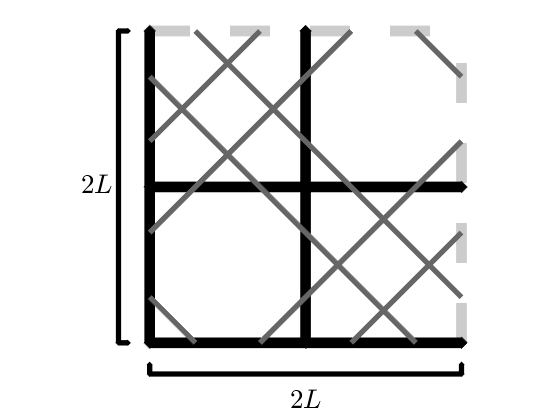
\includegraphics[width=0.4\linewidth]{SFig2.png}
    \caption{{\bf Unit cell for Design A.} This design is inspired by the sponge structure and consists of a square grid  reinforced by a double diagonal system. The horizontal and vertical struts have length $L$ and circular cross section with diameter $D_{A,nd}$ and, as with the sponge, we assume $D_{A,nd}/L=0.1$. The diagonal elements have a circular cross section  with diameter $D_{A,d}=2 D_{A,nd}$.}
    \label{DesignA}
\end{figure}

\subsubsection{Rectangular cross-section}
From $A_{nd}/A_d\approx 1.4$ we know that the volume is the same given that the in-plane dimension is constant, namely $V_{nd}/V_d\approx 1.4$. Assuming that the in-plane thickness is given by $t$, we can derive the following volumes for the diagonal and non-diagonal, respectively:
\begin{equation}
	V_{A,nd}=8LD_{A,nd}t
\end{equation}
\begin{equation}
	V_{A,d}=8\sqrt{2}LD_{A,d}t
\end{equation}
Let us enter this into our biological observation, which yields:
\begin{equation}
	\frac{V_{A,nd}}{V_{A,d}}\approx 1.4\approx\sqrt{2}=\frac{8LD_{A,nd}t}{8\sqrt{2}LD_{A,d}t}
\end{equation}
Therefore, we can simplify this relationship as
\begin{equation}
	D_{A,nd}=2D_{A,d}
\end{equation}

\subsection{Design B}
Design B is similar to the sponge design (Design A) and is likewise characterized by an alternation of open and closed cells (\cref{DesignB}). However, instead of having two diagonals offset from the nodes, here we only have one diagonal passing through the nodes and crossing every other cell. 
\subsubsection{Circular cross section}
It follows that the non-diagonal and diagonal volumes are given by
\begin{equation}
V_{B,nd}=V_{A,nd}=2\pi L D_{B,nd}^2
\end{equation}
and
\begin{equation}
V_{B,d}=2\sqrt{8} L \left(\pi \frac{{D}_{B,d}^2}{4}\right),
\end{equation}
respectively.
Using the constraints provided by \cref{con1} and \cref{con2}, as well as the above volumes, we  obtain 
\begin{equation}
{{D}_{B,nd}}={{D}_{A,nd}}
\end{equation}
and
\begin{equation}
\frac{{D}_{B,d}}{{D}_{B,nd}}=\frac{1}{\sqrt{2}}.
\end{equation}

\begin{figure}[H]
    \centering
    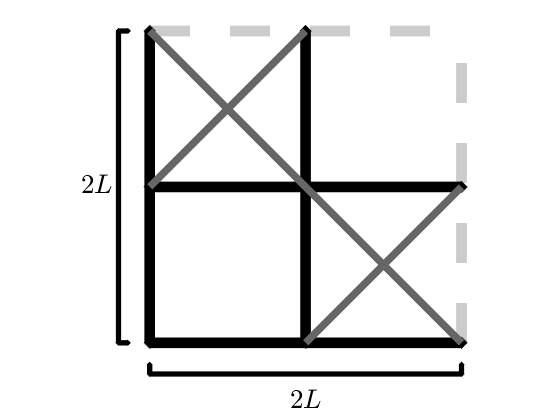
\includegraphics[width=0.4\linewidth]{SFig3.png}
    \caption{{\bf Unit cell for Design B.} This design is still characterized by an alternation of open and closed cells. However, instead of having two  diagonals offset from the nodes, here we only have one diagonal passing through the nodes and crossing every other cell. The horizontal and vertical struts have length $L$ and a circular cross section with diameter $D_{B,nd}$. The diagonal elements have a circular cross section  with diameter $D_{B,d}={D_{B,nd}}/{\sqrt{2}}$.}
    \label{DesignB}
\end{figure}

\subsubsection{Rectangular cross section}

For this design the volume of non-diagonal elements remain the same, namely,
\begin{equation}
		V_{B,nd}=8LD_{B,nd}t.
\end{equation}
However, the volume for the diagonal elements will is different as a result the change in total length, namely,
\begin{equation}
		V_{B,d}=4\sqrt{2}LD_{A,d}t.
\end{equation}
In in effort to maintain a constant volume ration between the diagonally reinforced designs, we use the same volume ratio as per observation
\begin{equation}
		\frac{V_{B,nd}}{V_{B,d}}\approx 1.4\approx\sqrt{2}=\frac{8LD_{B,nd}t}{4\sqrt{2}LD_{B,d}t}
\end{equation}
which simplifies to
\begin{equation}
	D_{B,nd}=D_{B,d}
\end{equation}
and
\begin{equation}
	D_{B,nd}=D_{A,nd}
\end{equation}

\subsection{Design C}
Design C is inspired by the town lattice truss design introduced by architect Ithiel Town in 1820 \citep{waddell1916} and consists of every cell being reinforced by diagonal trusses passing through the nodes (see \cref{DesignC}).

\subsubsection{Circular cross section}
For this design, the non-diagonal and diagonal volumes of the unit cell are given by:
\begin{equation}
V_{C,nd}=V_{A,nd}=2 L \pi D^2_{A,nd}
\end{equation}
and
\begin{equation}
V_{C,d}=V_{A,d}=2\sqrt{2}L \pi D^2_{A,d},
\end{equation}
respectively.
Using the constraints provided by \cref{con1} and \cref{con2} we  obtain 
\begin{equation}
{{D}_{C,nd}}={{D}_{A,nd}}
\end{equation}
and
\begin{equation}
\frac{{D}_{C,d}}{{D}_{C,nd}}=\frac{1}{2}.
\end{equation}

\begin{figure}[H]
    \centering
    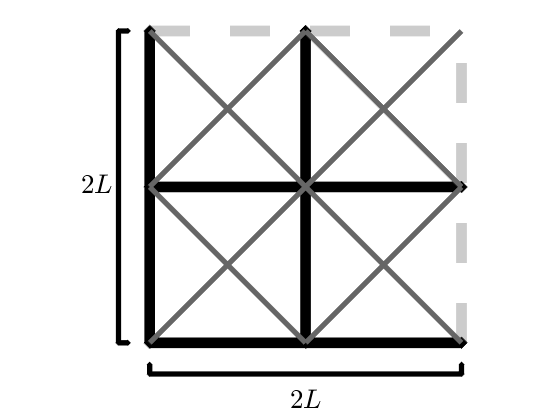
\includegraphics[width=0.4\linewidth]{SFig4.png}
    \caption{{\bf Unit cell for Design C.} This design consists of a square grid with all cells being reinforced by diagonal trusses passing through the nodes.  The horizontal and vertical struts have length $L$ and a circular cross section with diameter $D_{C,nd}$. The diagonal elements have a circular cross section  with diameter $D_{C,d}={D_{C,nd}}/{2}$.}
    \label{DesignC}
\end{figure}

\subsubsection{Rectangular cross section}
Because the total length of the diagonal and non-diagonal elements are the same as for Design A, we obtain the same diameters for the elements, namely,
\begin{equation}
D_{A,nd}=2D_{A,d}
\end{equation}
and
\begin{equation}
D_{C,nd}=D_{A,nd}
\end{equation}

\subsection{Design D} 
Design D comprises only the square grid without diagonal reinforcement (\cref{DesignD}) and is well known to be unstable and very limited in resisting shear forces \citep{gibson1999,deshpande2001}. As such, for this design we allocate the total material volume to the non-diagonal elements.

\subsubsection{Circular cross section}
Since
\begin{equation}
V_{D,T}=V_{D,nd}=V_{A,nd}=2\pi L D_{D,nd}^2,
\end{equation}
using the constraint provided by \cref{con1} we obtain
\begin{equation}
{D_{D,nd}}={D_{A,nd}}\sqrt{1+\frac{\sqrt{2}}{4}}. 
\end{equation}

\begin{figure}[H]
    \centering
    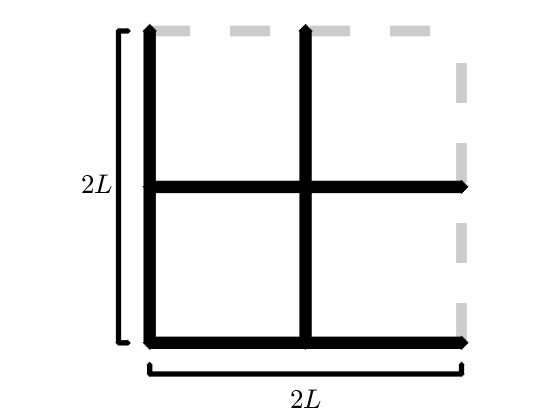
\includegraphics[width=0.4\linewidth]{SFig5.png}
    \caption{{\bf Unit cell for Design D.} This design consists of a square grid without diagonal reinforcement.  The horizontal and vertical struts have length $L$ and a circular cross section with diameter $D_{D,nd}$.}
    \label{DesignD}
\end{figure}

\subsubsection{Rectangular cross-section}
For this design, because it does not contain any diagonal elements, we must allocate the total volume of the structure fully on the non-diagonal elements. Thus we can formulate the total volume of Design A as
\begin{equation}
	V_{A,nd}+V_{A,d}=(D_{A,nd}+\sqrt{2}D_{A,d})8Lt
\end{equation}
Using the relationship between the non-diagonal thickness and diagonal thickness, we obtain
\begin{equation}
V_{A,nd}+V_{A,d}=\left(1+\frac{1}{\sqrt{2}}\right)8LtD_{A,nd}
\end{equation}

We can build a relationship between Design A and Design D through the total volume, such that the total volume of Design A is the same as the total volume of Design D
\begin{equation}
\left(1+\frac{1}{\sqrt{2}}\right)8LtD_{A,nd}=8LtD_{D,nd}
\end{equation}
which yields a relationship between the thicknesses of the non diagonal elements as
\begin{equation}
	D_{D,nd}=\left(1+\frac{1}{\sqrt{2}}\right)D_{A,nd}
\end{equation}

\section{Numerical Model}
The finite element analysis presented in this article was conducted using the {\it ABAQUS 2017} implicit scheme. For all buckling analysis, we performed a linear stability buckling analysis and for all stiffness results we performed a linear elastic analysis. All elements are assumed to be 1D Timoshenko beam elements and all beam crossings are assumed to be welded joints. The model assumes a linear elastic material with standard Poisson's ratio $\nu=0.3$ and a non-dimentionalized elastic Young's modulus of $E=1$ (resulting in all values of stresses being non-dimentionalized by the material's Young's modulus).

For the boundary conditions, we treat the geometries from the previous section as Representative Volume Elements (RVE) which are used to generate infinite structures. To implement the infinite numerical scheme, we define periodic boundary conditions along the perimeter of the RVE. Each RVE is subjected to a macroscopic deformation gradient, so that 
\begin{equation}
	\boldmath u_B-u_A=(\bar{F}-I)(X_B-X_A),
\end{equation}
where $A$ and $B$ are a pair of nodes located on the opposite side of the structure and $\boldmath u_X$ represents the finite displacement of node $X$. The deformation boundary conditions can thus be imposed on the deformation gradient given by $(\mathbold{\bar{F}-I})$, which are viewed as generalized degrees of freedom operationally applied using a set of virtual nodes. \citep{danielson2002}.

For each instance, seeding of the mesh was chosen to be at least 1/10 of the minimum beam length. 

\section{Optimization Analysis}
For the optimization portion of the work presented in the main article we use a stochastic, derivative-free evolutionary method called Covariance Matrix Adaptation Evolution Strategy (CMA-ES) implementation in Python \citep{hansen2003}. The algorithm parameters (continuous input variables) are: the structure's mass ratio $\lambda$ (keeping the total structure volume constant, as well as distributing the mass evenly through all diagonal and non-diagonal elements respectively) and the separation of the even numbered diagonal elements from the non-diagonal junction. Separate instances of the optimization algorithm are analyzed for different numbers of diagonal reinforcements. For simulations with odd number of diagonal reinforcements, only an even number of diagonals are separated while keeping one diagonal going through the non-diagonal junction in order to ensure geometry symmetry. 

The algorithm's initial values are chosen to be in the center of the design space, namely, $\lambda=1$ and diagonal separation$=0.5*L$. The covariance matrix is initialized uniformly with standard deviation ($\sigma$) half of the domain space, which are normalized to remain between 0 and 1. The optimization is run for uniaxial loading condition in the direction parallel to the non-diagonal elements. 

For the optimization results presented in the main article, we seek to maximize the critical buckling load using a single objective target function. However, an equivalent analysis is performed to maximize the critical buckling strain as the target response (\cref{BucklingOptimization}.) 

\begin{figure}[H]
    \centering
    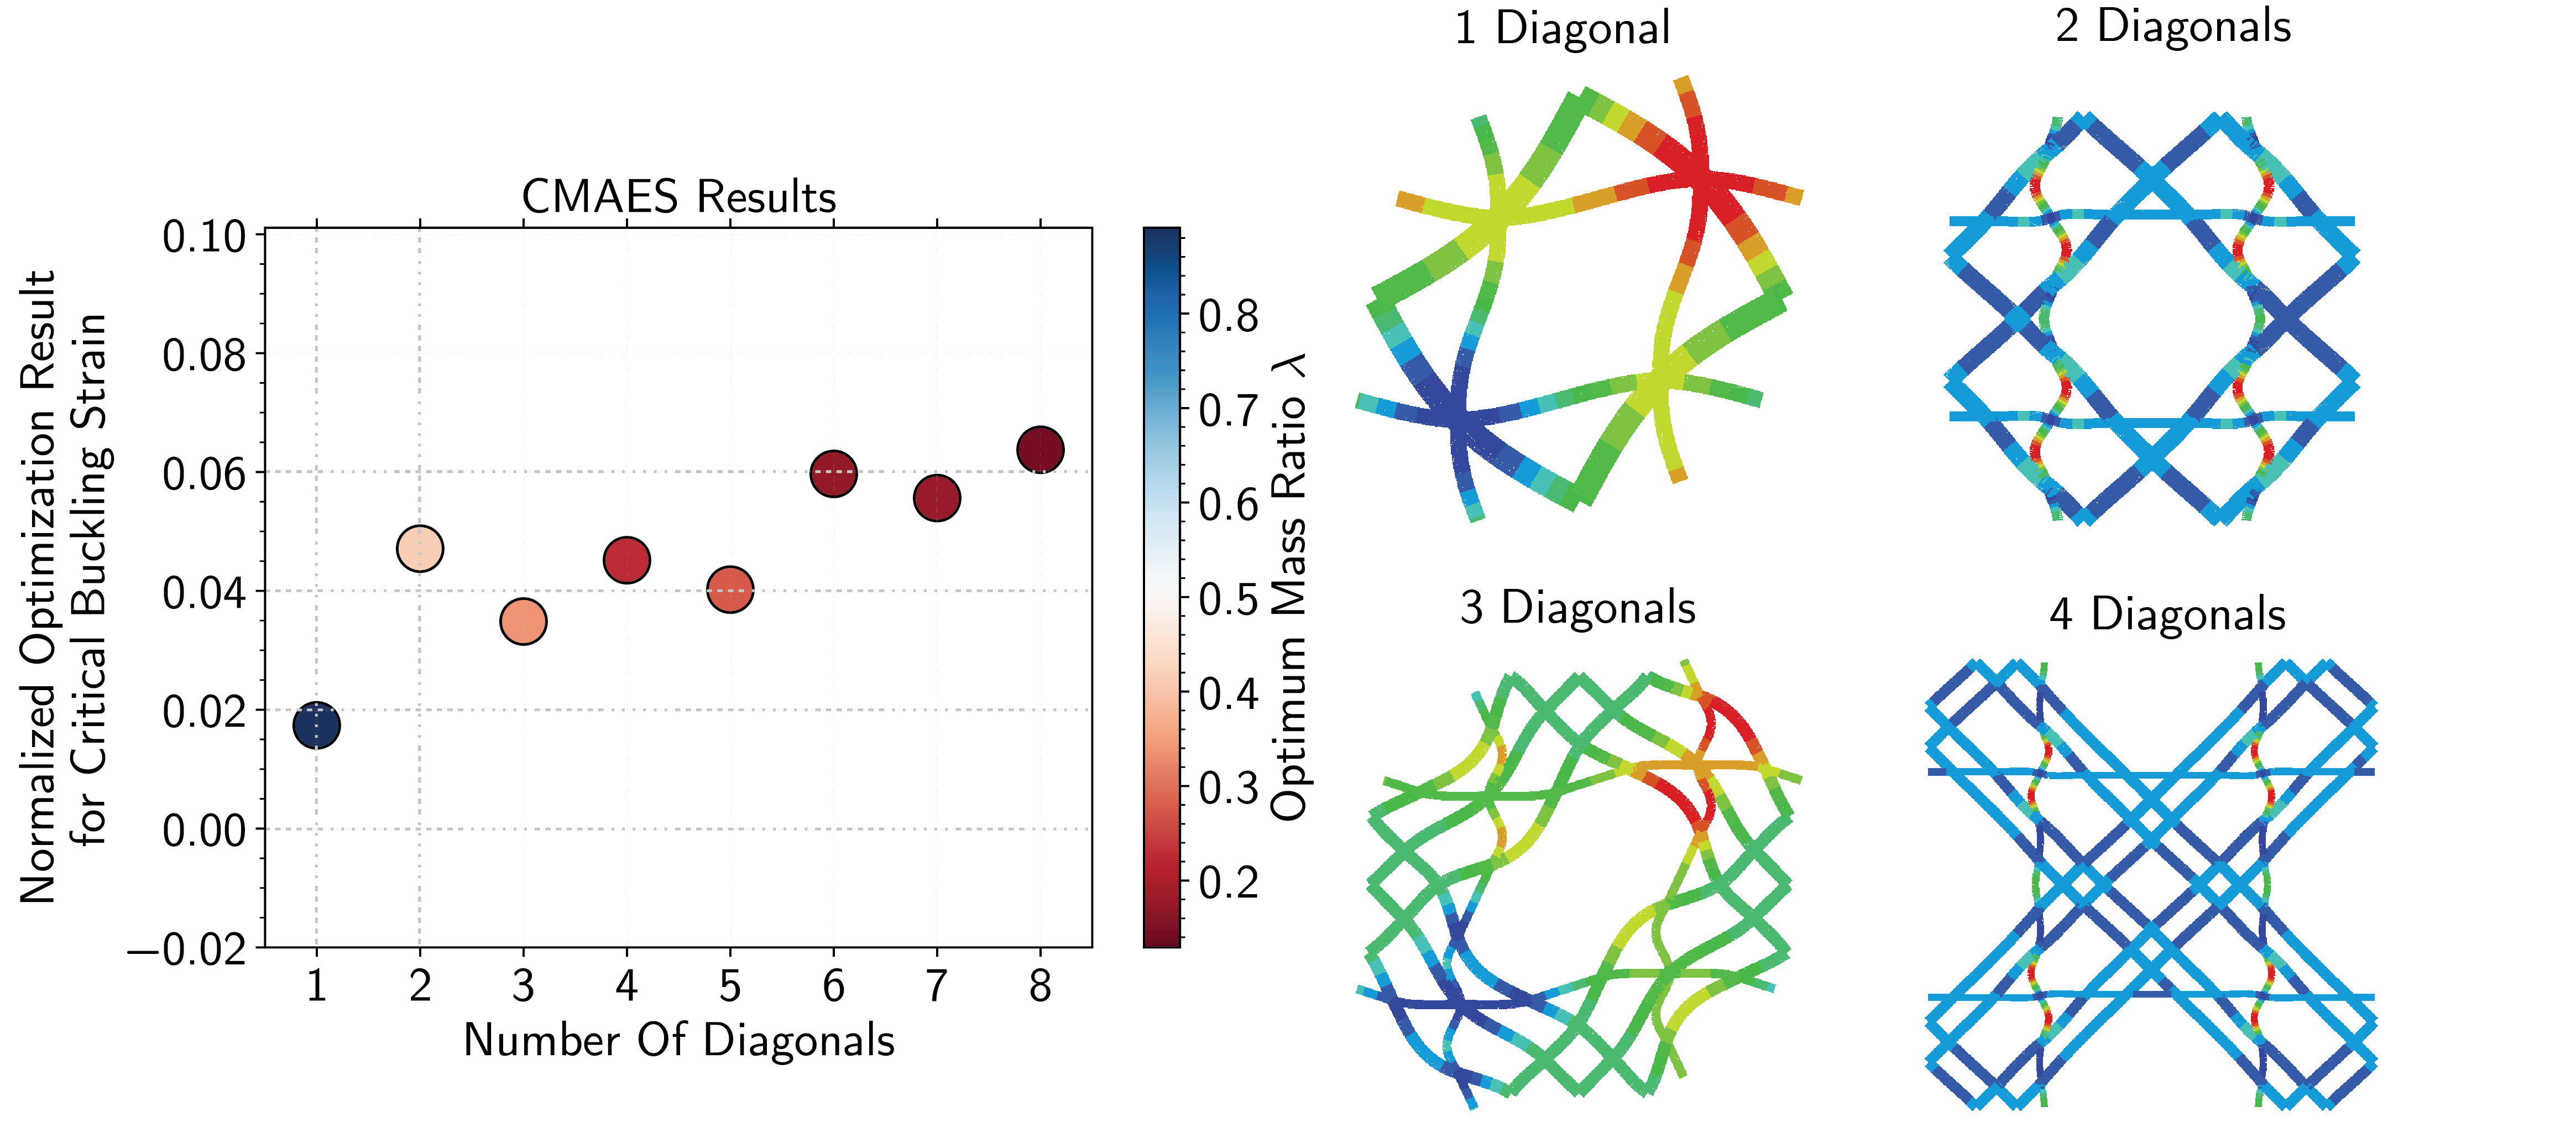
\includegraphics[width=0.9\linewidth]{SFig6.png}
    \caption{{\bf Buckling Optimization.} Graph shows optimal value of critical buckling strain for varying number of diagonals. For all simulations, the total mass of the structure is maintained constant while the mass-ratio is allowed to vary. Furthermore, the diagonal separation for each pair of diagonal is allowed to vary together ensuring half symmetry of the structure at all times. The optimization is run under a uniaxial loading condition. The color of each point on the graph corresponds to the optimum value of mass ratio for that particular number of diagonals. Four deformation plots of the optimum structure and buckling modes are provided on the right for their respective number of diagonals.}
    \label{BucklingOptimization}
\end{figure}

\section{Circular Cross-Section Results}
The results presented here complement that found on the main article and show that the structural benefit for the Design A persists when using a different cross-section for the structure. We show that for varying loading angles all of the diagonally reinforced designs provide the same stiffness, but Design A consistently provides the best resistance to buckling. 

\begin{figure}[H]
	\centering
	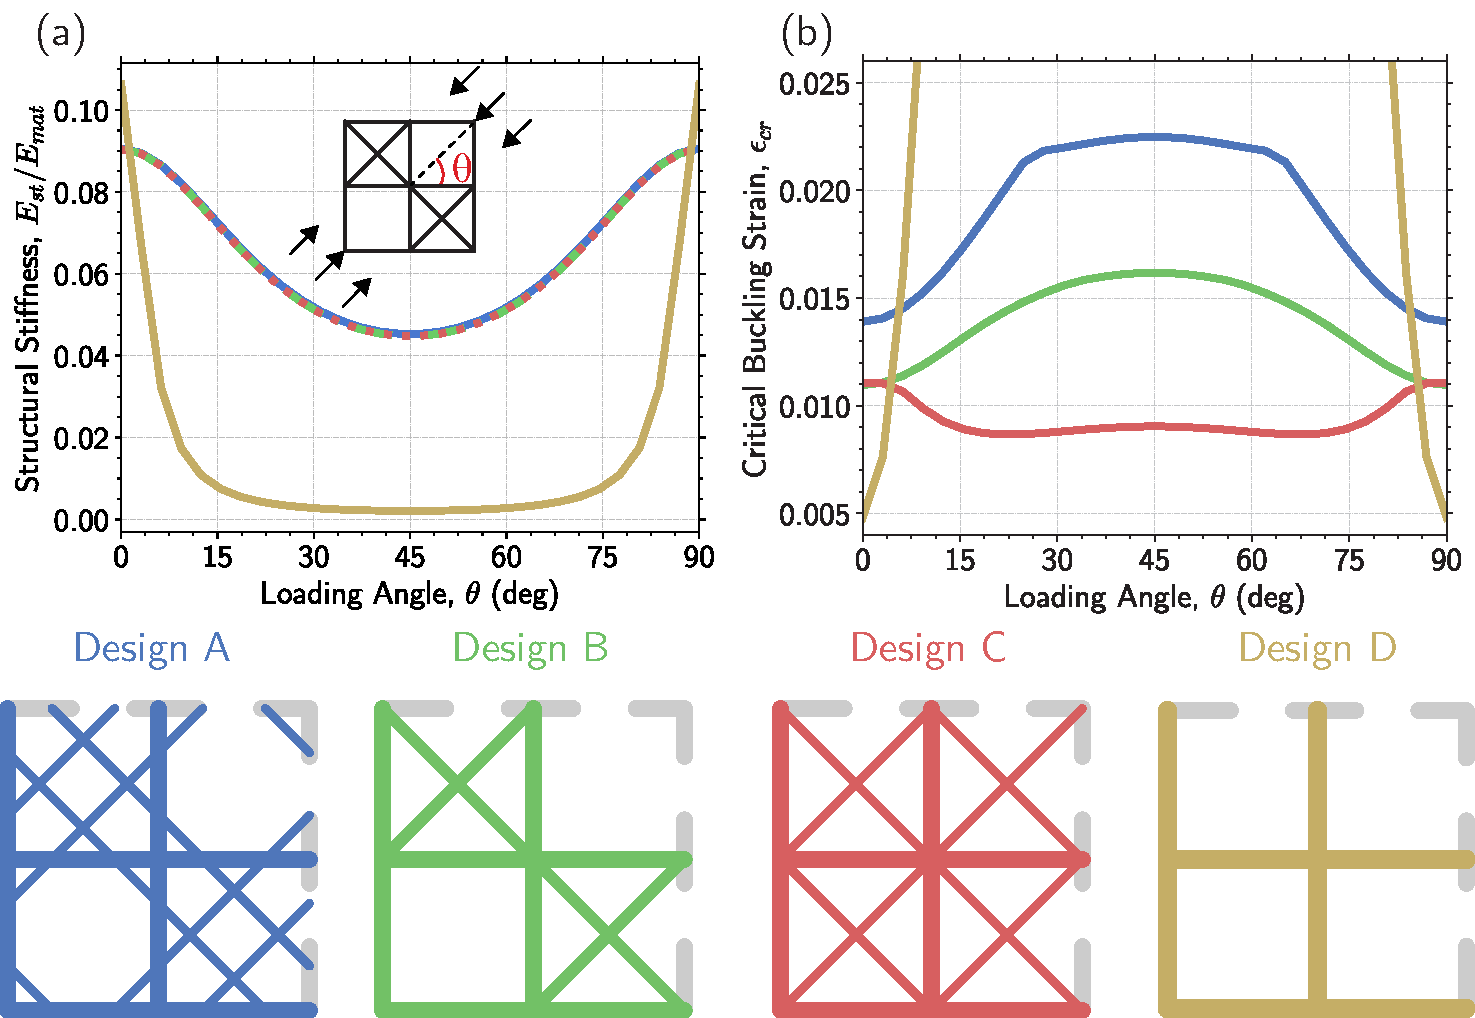
\includegraphics[width=0.6\linewidth]{SFig7.pdf}
	\caption{{\bf Circular Cross Section Results.} The color of the lines correspond to it's respective design color below the plots. (a) Shows the linear elastic stiffness of the different designs as a function of the loading angle. All structures except for the design without diagonal reinforcement have the same stiffness. (b) Shows the critical buckling strain for varying loading angle. For all angles, Design A outperforms other diagonally reinforced designs. These results show that the two diagonal benefit persists beyond a particular beam cross-section design.}
	
	\label{CircularCrossSection}
\end{figure}
\section{Parameter Exploration}
In order to survey the design space of the double diagonal construction we explore parametric simulations for 2 variables: diagonal separation and mass ratio. For each of these separate analysis, we maintain the sponge geometry as our base geometry and vary only the respective variable. 

\subsection{Rectangular Cross Section}
This section shows the results when using a rectangular cross-section for the truss members. From \cref{SquareCrossSectionParameter}(a) it is apparent that there exists an optimum for the diagonal separation that occurs when the spacing between diagonals are approx 0.2 of the horizontal distance between vertical struts. This optimum value also persists when varying the loading angle. From \cref{SquareCrossSectionParameter}(b) it can be seen that the linear stiffness is symmetrically and almost purely dependent on the mass ratio allocated to diagonal versus non-diagonal elements. Comparing this figure to \cref{CircularCrossSectionParameter}(b) we can also see that even the design cross-section does not change the linear stiffness behavior. 

\begin{figure}[H]
	\centering
	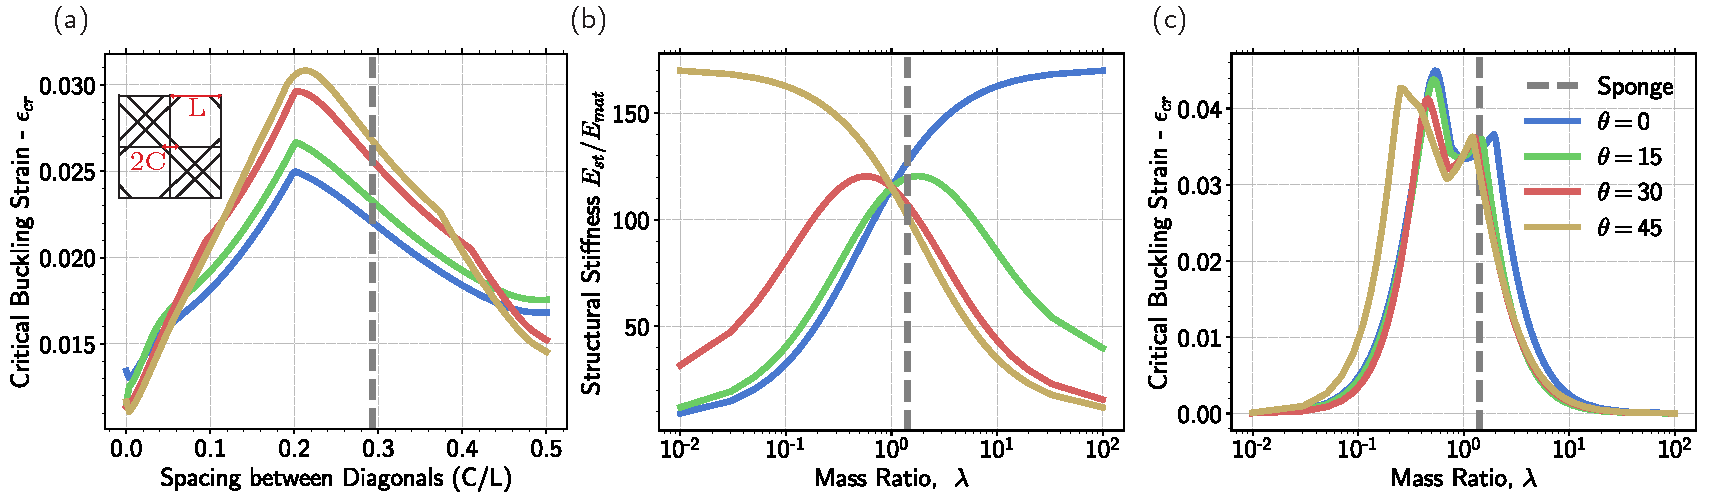
\includegraphics[width=0.9\linewidth]{SFig8.pdf}
	\caption{{\bf Rectangular Cross Section Parameter Exploration.} For each of these plots, we vary a single parameter while maintaining the base sponge inspired geometry constant. The gray line indicates the sponge design parameter. (a) Shows the critical buckling strain for varying spacing between diagonals. (b) Shows the structural stiffness of the geometry as we vary the mass ratio $\lambda$. (c) Shows the critical buckling strain of the geometry as we vary the mass ratio $\lambda$.}
	\label{SquareCrossSectionParameter}
\end{figure}

\subsection{Circular Cross Section}
\begin{figure}[H]
	\centering
	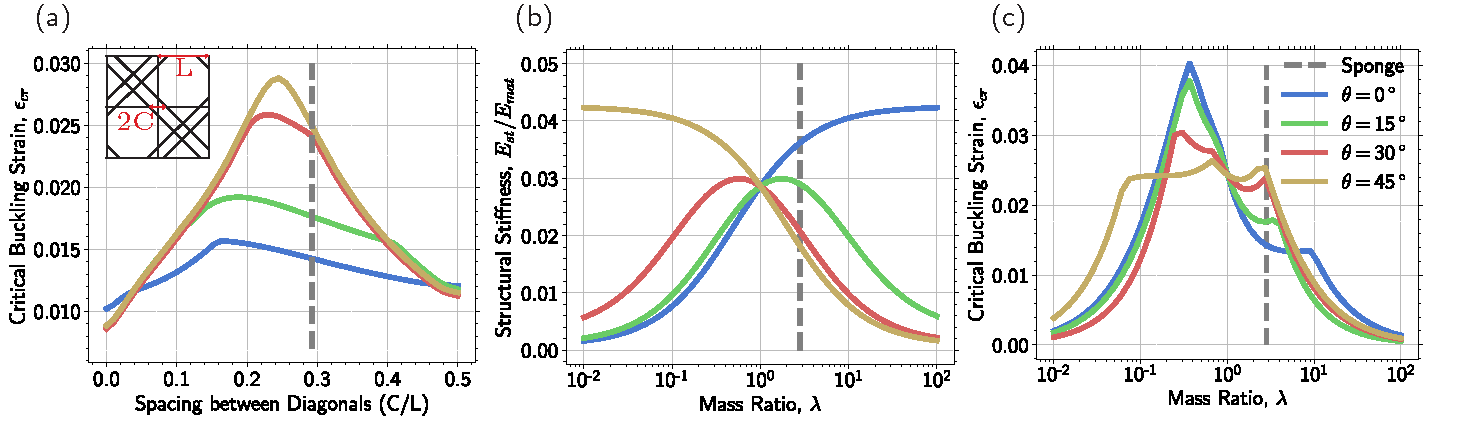
\includegraphics[width=0.9\linewidth]{SFig9.pdf}
	\caption{{\bf Circular Cross Section Parameter Exploration.} For each of these plots, we vary a single parameter while maintaining the base sponge inspired geometry constant. The gray line indicates the sponge design parameter. (a) Shows the critical buckling strain for varying spacing between diagonals. (b) Shows the structural stiffness of the geometry as we vary the mass ratio $\lambda$. (c) Shows the critical buckling strain of the geometry as we vary the mass ratio $\lambda$.}
	\label{CircularCrossSectionParameter}
\end{figure}


\section{Local and Global Instabilities}
For infinite structures modeled using period boundary conditions, it is important to realize the distinction between local instabilities (i.e. instabilities with wavelength that are of the order of the size of the unit cell) and global instabilities (i.e. instabilities with large wavelengths in comparison to the size of the unit cell). In order to capture any global instabilities potentially missed by using the minimum RVE, we further develop our period numerical studies to include RVEs that tessellate the unit cells presented in \cref{sec:designs}. For all designs, we increase the domain size by tessellating up to 20x20 unit cells (creating a base grid of 40x40 square cells). For Designs A-C, the critical bucking strain and modes do not change for larger unit cells suggesting that there does not exist a global instability. Whereas, for Design D, as we increase the domain size (add more unit cells to the tessellation), the instability  wavelength continues to grow with the size of the domain, suggesting a global macroscopic instability that depends on the size of the domain. The critical buckling strain is inversely proportional with the RVE size and approaches 0 in the limit that the RVE size approaches infinity. It is well known and documented that Design D is unstable when loaded in uniaxial compression. 

\mf{Write about minimum RVE -- how do I convey this message? Should I produce a plot or just verbally state this check?}

% Bibliography
\nocite{aizenberg2005}
\nocite{deshpande2001}
\nocite{miserez2008}
\nocite{weaver2010}

\bibliography{refs}
\bibliographystyle{apalike}
% \bibliographystyle{plainnat}

\end{document}